\documentclass[a4paper]{article}

\usepackage[utf8]{inputenc}
\usepackage[T1]{fontenc}
\usepackage{textcomp}
\usepackage{listings}
\usepackage{lmodern}
\usepackage{amsfonts}
\usepackage{titling}
\usepackage{lipsum}
\usepackage[left=1in, right=1in, bottom=1in, top=1in]{geometry}
\usepackage{amsthm}
\usepackage{tcolorbox}
\usepackage{hyperref}
\usepackage{xcolor}
\usepackage{graphicx}
\usepackage{makeidx}
\usepackage{tikz}
\usepackage{cases}
\usepackage{apacite}
\usepackage{tkz-berge}
\usepackage{url}
\usepackage{tgtermes}
\usepackage{sectsty}
\usepackage{subcaption}
\usepackage{setspace}
\usepackage{float}
\usepackage{amsmath, amssymb}


% figure support
\usepackage{import}
\usepackage{xifthen}
\pdfminorversion=7
\usepackage{pdfpages}
\usepackage{transparent}
\usepackage{color}
\newcommand{\incfig}[2][1]{%
    \def\svgwidth{#1\columnwidth}
    \import{./figures/}{#2.pdf_tex}
}

%mathstyling
\theoremstyle{plain}
\newtheorem{thm}{Theorem}[section]
\newtheorem{lem}[thm]{Lemma}
\newtheorem{prop}[thm]{Proposition}
\newtheorem*{cor}{Corollary}

\theoremstyle{definition}
\newtheorem{defn}{Definition}[section]
\newtheorem{conj}{Conjecture}[section]
\newtheorem{exmp}{Example}[section]
\newtheorem{axiom}{Axiom}
\theoremstyle{remark}
\newtheorem*{rem}{Remark}
\newtheorem*{note}{Note}

\definecolor{darkgreen}{rgb}{0.0, 0.5, 0.0}

\pdfsuppresswarningpagegroup=1
\lstset{
tabsize = 4, %% set tab space width
showstringspaces = false, %% prevent space marking in strings, string is defined as the text that is generally printed directly to the console
numbers = left, %% display line numbers on the left
commentstyle = \color{darkgreen}, %% set comment color
keywordstyle = \color{blue}, %% set keyword color
stringstyle = \color{red}, %% set string color
rulecolor = \color{black}, %% set frame color to avoid being affected by text color
basicstyle = \small \ttfamily , %% set listing font and size
breaklines = true, %% enable line breaking
numberstyle = \tiny,
  frame=none,
  xleftmargin=2pt,
  stepnumber=1,
  belowcaptionskip=\bigskipamount,
  captionpos=b,
  escapeinside={*'}{'*},
  language=haskell,
  tabsize=2,
  emphstyle={\bf},
  showspaces=false,
  columns=flexible,
  showstringspaces=false,
  morecomment=[l]\%,
}
\begin{document}
	\begin{titlepage}
	\begin{center}
	\large
	University of Warwick \\
	Department of Computer Science \\
	\huge
	\vspace{50mm}
	\rule{\linewidth}{0.5pt} \\
	CS139 \\
	\vspace{5mm}
	\Large
	Web Development Technologies
	\rule{\linewidth}{0.5pt}
	\vspace{5mm}
	\begin{figure}[H]
	\centering
	
\includegraphics[width=0.4\textwidth]{crest.eps}
	\end{figure}
	\vspace{37mm}
	Cem Yilmaz \\
	\today
	\end{center}
	\end{titlepage}
	\newpage
	\tableofcontents
	\newpage
\section{HTML}
\subsection{Syntax}
HTML stands for HyperText Markup Language and is semantic. This means that it describes the structure of the document and not the content. It is intended to modify the appearance of HTML elements and can be in fact frustrating to use for page layouts.

A lot of HTML is done with the $<>$ brackets. For example,
\begin{lstlisting}[language = HTML , caption={Heading} , frame = trBL , firstnumber = last , escapeinside={(*@}{@*)}]
<h1>Welcome to CS139</h1>
\end{lstlisting}
This would set the header tag to the text "Welcome to CS139". For this module, we will be using JSFiddle, that is available online.
\subsubsection{Doctypes}
Every HTML documents should have a doctype definition on top. In particular, HTML5 uses
\begin{lstlisting}[language = HTML , caption={DOCTYPE} , frame = trBL , firstnumber = last , escapeinside={(*@}{@*)}]
<!DOCTYPE html>
\end{lstlisting}
It helps the browser to know what to expect.
\subsubsection{Example HTML5 Document}
\begin{lstlisting}[language = HTML , caption={Example Document} , frame = trBL , firstnumber = last , escapeinside={(*@}{@*)}]
<!DOCTYPE html>
<html>

	<head>
		<meta charset="UTF-8">
		<title>Title for Hello World </title> // Title that is seen at the top of the browser
	</head>
	<body>
		<h1>Hello world</h1> // Biggest header for the website
	</body>
</html>
\end{lstlisting}
\subsubsection{Head tag}
This tag is used by the browser, web-crawlers and bots. IT includes meta-tags required by these applications and includes location of supporting documents e.g. JavaScript and CSS.
\subsubsection{Text-encoding}
Familiar with ASCII, but that is only $128$ characters. In particular, UTF-8 has 107000 characters and is denoted with
\begin{lstlisting}[language = HTML , caption={Text-encoding} , frame = trBL , firstnumber = last , escapeinside={(*@}{@*)}]
<meta>
\end{lstlisting}
\subsubsection{Body tag}
This is the tag where main information goes into that the user gets to read. Its syntax is 
\begin{lstlisting}[language = HTML , caption={Body} , frame = trBL , firstnumber = last , escapeinside={(*@}{@*)}]
<body>
</body>
\end{lstlisting}
\subsubsection{Syntax}
\begin{lstlisting}[language = HTML , caption={Syntax} , frame = trBL , firstnumber = last , escapeinside={(*@}{@*)}]
<a href="google.com">Google search</a>
\end{lstlisting}
In the code above, $a$ is the element name. The hyperlink in href is called the \textit{Attribute}. The content is the \textit{Google search} text.
However, there are also empty tags e.g.
 \begin{lstlisting}[language = HTML , caption={Empty Tag} , frame = trBL , firstnumber = last , escapeinside={(*@}{@*)}]
<meta charset="utf-8">
\end{lstlisting}
\subsubsection{Nesting Definitions}
\begin{tcolorbox}[colback=black!3!white,colframe=black!60!white,title=\begin{defn}Child and parent \label{Child}\end{defn}]
A syntax is a child if and only if there exists a tag that is at a lower level than the upper tag.
\begin{lstlisting}[language = HTML , caption={Parent Child} , frame = trBL , firstnumber = last , escapeinside={(*@}{@*)}]
<body>
	<p>
	This is some text
	</p>
</body>
\end{lstlisting}
In particular, $<body>$ is the parent of $<p>$ and $<p>$ is the child of $<body>$.
\end{tcolorbox}
\begin{tcolorbox}[colback=black!3!white,colframe=black!60!white,title=\begin{defn}Sibling \label{Sibling}\end{defn}]
Sibling is when the tag is on the same level. For example,
\begin{lstlisting}[language = HTML , caption={Sibling} , frame = trBL , firstnumber = last , escapeinside={(*@}{@*)}]
<body>
	<p>
	This is some text
	</p>
	<p>
	Another text
	</p>
</body>
\end{lstlisting}
In here, the $p$ are siblings.
\end{tcolorbox}
Similarly, the term descendants would be group of tags of in comparison to a tag that is a parent of all.
\subsubsection{Lists}
There are 3 types of lists:
\begin{itemize}
	\item Ordered lists denoted with $<ol>$ and then listed items with $<li>$ 
	\item Unordered lists denoted with $<ul>$ and then listed items with $<li>$ 
	\item Description list would list terms and then list descriptions. In particular, the tags that are used are $<dl>$, $<dt>$ and $<dd>$ which are list, item and description respectively.You can also created nested list if you simply begin another list inside a list.
		
\end{itemize}
For example
\begin{lstlisting}[language = HTML , caption={Lists} , frame = trBL , firstnumber = last , escapeinside={(*@}{@*)}]
<ul>
	<li> shopping </li>
	<ol>
		<li> eggs </li>
		<li> bread </li>
	</ol>
	<li> cooking </li>
</ul>
\end{lstlisting}
\subsubsection{Hyperlinks}
\begin{flushleft}
Hyperlinks are listing websites to a specific piece of text. For example
\begin{lstlisting}[language = HTML , caption={Hyperlink} , frame = trBL , firstnumber = last , escapeinside={(*@}{@*)}]
<a href="www.google.com"> This is google hyperlink </a>
\end{lstlisting}
You can also hyperlink inside the website using ids. For example,
\begin{lstlisting}[language = HTML , caption={IDs} , frame = trBL , firstnumber = last , escapeinside={(*@}{@*)}]
<body>
<h1> Links </h1>
<p id = "#top">
	This is some paragraph text
</p>
<a href="#top"> Go to top </a>
\end{lstlisting}
\subsubsection{Images}
You can also include images with a singular tag that use the $src$ and $alt$ attributes.
For example,
\begin{lstlisting}[language = HTML , caption={Image embed} , frame = trBL , firstnumber = last , escapeinside={(*@}{@*)}]
<img src="http://warwick.ac.uk/logo.gif" alt="Warwick Logo" title="Warwick Logo" width=200 height=60 />
\end{lstlisting}
\subsubsection{Character entities}
\begin{lstlisting}[language = HTML , caption={Character entities} , frame = trBL , firstnumber = last , escapeinside={(*@}{@*)}]
&nbsp; //Nonbreakable space
&lt; //<
&gt; //>
&copy; //Copyright symbol
&trade; //Trademark symbol
\end{lstlisting}
\subsubsection{Break Line}
You can get a new line or break a line using the tag
\begin{lstlisting}[language = HTML , caption={Break} , frame = trBL , firstnumber = last , escapeinside={(*@}{@*)}]
<br>
\end{lstlisting}
\subsection{Semantic Mark-up}
Some semantics include but are not limited to
\begin{lstlisting}[language = HTML , caption={Semantics} , frame = trBL , firstnumber = last , escapeinside={(*@}{@*)}]
<abbr>
<cite>
<time>
<span>
<div>
\end{lstlisting}
That is, these do not change the looks but are important regardless. Usually, semantic mark-up refers to creating IDs on code to give meaning to piece of text and make it readable. In particular, the example in Hyperlinks with the ID is an example of a semantic mark-up.
\subsection{Validation}
You can make sure that your HTML is valid using a validation tool provided by W3C. The website is \link{http://validator.w3.org}
\subsection{Types of Style Sheet}
There are three different types of style sheet:
\begin{itemize}
	\item Author created style sheets
	\item User style sheets
	\item Browser style sheets
\end{itemize}
\subsection{Tables}
A lot of data in HTML conveys data in rows and columns, i.e., a table. 
\begin{lstlisting}[language = HTML , caption={Table} , frame = trBL , firstnumber = last , escapeinside={(*@}{@*)}]
<table>
	<tr>
		<td> The death of Marata </td>
		<td> Jacques-Louis David </td>
		<td> 1793 </td>
		<td> 162cm </td>
		<td> 128cm </td>
	</tr>
	<tr>
		<td> Burial at Ornans </td>
		<td> Gustave Courbet </td>
		<td> 1849 </td>
		<td> 314cm </td>
		<td> 663cm </td>
	</tr>
</table
\end{lstlisting}
In here, $</tr>$ stands for table row. $<td>$ stands for table data. Therefore cells in a row are declared by td, whereas rows are declared by tr. There is also $<th>$ which characterises table header. You can also add rowspan i.e.
\begin{lstlisting}[language = HTML , caption={Rowspan} , frame = trBL , firstnumber = last , escapeinside={(*@}{@*)}]
<table>
	<tr>
		<th> Artist </th>
		<th> Title </th>
		<th> Year </th>
	</tr>
	<tr>
		<td rowspan="3"> Jacques-Louis David </td>
		<td> The death of Marat </td>
		<td> 1793 </td>
	</tr>
	<tr>
		<td> The Intervention of Sabine Woman </td>
		<td> 1789 </td>
	</tr>
	<tr>
		<td> Napoleon Crossing the Alps </td>
		<td> 1800 </td>
	</tr>
</table>
\end{lstlisting}
Column span works in a similar fashion. Furthemore
\begin{lstlisting}[language = HTML , caption={Table Head and Footer} , frame = trBL , firstnumber = last , escapeinside={(*@}{@*)}]
<thead>
// Top of the table. It is always the top rows of a table.
</thead>
<tbody>
// Middle of the table. It is always inbetween header and foot.
<tbody>
<tfoot>
// Sets the last row of the table. This will always be at the bottom of the table.
</tfoot>
\end{lstlisting}
\subsection{Forms}
Sometimes we require to get data from the user, e.g. log-in page. It has the attributes:	
\begin{itemize}
	\item Action - the destination of the form data when submitted
	\item Method - the way in which the data is sent (GET or POST)
	\item Accept-charset - The charset accepted by the form
\end{itemize}
\begin{lstlisting}[language = HTML , caption={A basic form} , frame = trBL , firstnumber = last , escapeinside={(*@}{@*)}]
<form method="post" action="process">
	<fieldset>
		<legend> Details </legend>
		<p>
			<label> Title: </label>
			<input type="text" name="title> />
		</p
		<p>
			<label> Country: </label>
			<select name="where">
				<option> Choose a country </option>
				<option> Canada </option>
				<option> Finland </option>
				<option> United States </option>
			</select>
		</p>
		<input type ="submit" />
	</fieldset>
</form>
\end{lstlisting}
\subsubsection{Attributes}
\begin{itemize}
	\item Type - the kind of input to accept
	\item Name - the name submitted to the server
	\item The value that you want the field to have
	\item Other attributes related to type...
\end{itemize}
\begin{lstlisting}[language = HTML , caption={Attributes} , frame = trBL , firstnumber = last , escapeinside={(*@}{@*)}]
<input type="text" name="city name" value="Warwick" >
<input type="text" name="uname" placeholder="what is your name" >
\end{lstlisting}
\subsubsection{Radio Buttons}
Radio buttons must have the same name in a group and allows you to select only a singular option
\begin{lstlisting}[language = HTML , caption={Radio Buttons} , frame = trBL , firstnumber = last , escapeinside={(*@}{@*)}]
<input type="radio" name="where" value="1">Coventry<br>
<input type="radio" name="where" value="2" checked>Warwick<br>
<input type="radio" name="where" value="3">Nottingham<br>
\end{lstlisting}
\subsubsection{Dropdown menus}
Dropdowns need $<option>$ elements with the $<select>$.
\begin{lstlisting}[language = HTML , caption={Dropdown menus} , frame = trBL , firstnumber = last , escapeinside={(*@}{@*)}]
<select name="choices">
	<option>First</option>
	<option selected>Second </option>
	<option> Third </option>
</select>	
\end{lstlisting}	
\subsubsection{Accessibility}
Sometimes we prefer the use of tables for data, not layout. In these cases, we use the caption element. This connect cells with a textual description in the header. You can also use "id" and "label for" to easen the accessability
\section{Introduction to Python/Flask}
\subsection{Flask and Python}
Flask is a server-side web micro-framework and it mainly uses Python as its scripting language. Its extensions provide further functionality. For example,
\begin{itemize}
	\item Dynamic HTML markup uses Jinja2
	\item Database access via SQLAchamy
	\item OThers such as Flask-WTF (forms) and Flask-Login (authentication)
\end{itemize}
It was released in 2010 and its version $2.0.2$ was released in October. Reddit, Linkedin, Netflix and Pinterest use it.
\subsection{General Architecture}
Python code is executed on a server and the output html is then sent to the client's browser.
\begin{figure}[H]
	\centering
	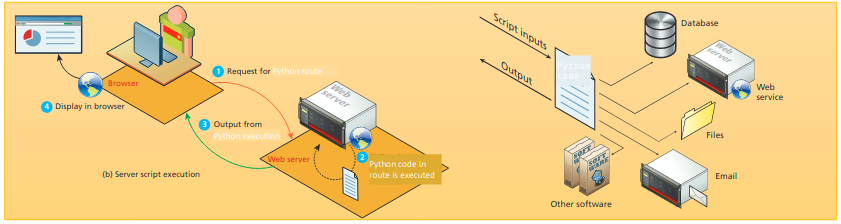
\includegraphics[width=0.8\textwidth]{architecture.png}
	\caption{Architecture of web server}
	\label{fig:architecture-png}
\end{figure}
\subsection{Flask and Python}
=Python is used to execute a web server and is written within a .py file. HTMl code is written in .html file. Python uses indentation for scoping without braces or semicolons. Comments use ectomorph simple or triple apostrophes e.g.
\begin{lstlisting}[language = Python , caption={Commenting} , frame = trBL , firstnumber = last , escapeinside={(*@}{@*)}]
# comment
''' comment '''
\end{lstlisting}
\subsection{Variable Naming}
Variables are duck=typed, i.e. dynamically and an integer. Variable names must begin with a letter or an underscore and cannot have spaces. Case sensitive value is not equal Value.
\subsection{Python Data Types}
Scalar types include
\begin{itemize}
	\item Integer
	\item Float
	\item Complex
	\item Boolean
	\item String
\end{itemize}
And compound types
\begin{itemize}
	\item Dictionary
	\item List and tuples
	\item Set
	\item Object
\end{itemize}
\subsection{Python Containers}
Python has $4$ containers types: Lists, Sets, Dictionaries and Tuples.
\begin{itemize}
	\item Lists are ordered and mutable, uses $[]$
	\item Sets are unordered and cannot have duplicates, uses $set\left(  \right) $ 
	\item Tuples are ordered and immutable, uses $(,)$ 
	\item Dictionaries are associative arraways - unordered values are references by their key, use $\{\}$
\end{itemize}
In particular, for examples, dictionaries can have "keys", e.g.
\begin{lstlisting}[language = Python , caption={Keys} , frame = trBL , firstnumber = last , escapeinside={(*@}{@*)}]
ages = {"Adam":27, "Dean":20, "Louise":30}
\end{lstlisting}
Then,
\begin{lstlisting}[language = Python , caption={Keys 2} , frame = trBL , firstnumber = last , escapeinside={(*@}{@*)}]
ages["Adam"] = 27
ages.update("Dean",20)
\end{lstlisting}
The key, which is their name, is linked to data which is their age.
\subsection{Python Functions}
You can define your own functions so that code is reusable. It is essentially creating methods. The code is
\begin{lstlisting}[language = Python , caption={Functions} , frame = trBL , firstnumber = last , escapeinside={(*@}{@*)}]
def <function name> (arg1, arg2...):
\end{lstlisting}
And these can return any object.
\subsection{Dealing with Forms}
Form values are submitted via a GET or POST method.
\begin{itemize}
	\item GET - encodes the parameters in the url, some of you have already discovered this
	\item POST - encodes form values in the message body.
\end{itemize}
Flask stores these values in the args(GET) or the form(POST) of the request object and we can pull out the values and do whatever we wish with them.
\subsection{Templates in Flask}
Web pages don't need to be created in Python and we can create HTML pages and render them from Python instead. An HTML page in Flask is called a Template and is stored in the Templates folder. IT is rendered using
\begin{lstlisting}[language = Python , caption={Template Render} , frame = trBL , firstnumber = last , escapeinside={(*@}{@*)}]
render_template(<pagename>)
\end{lstlisting}
And these templates have Jinja2 scripting. That is, these are not just HTML and they can be scripted and accept data from Python. For example,
\begin{itemize}
	\item Statements/scripts are written in $\{ \% \% \}$
	\item Expressions evaluated to the output are written in  $\{\{\} \} $ 
	\item Comments are written in $\{\# \#\} $
\end{itemize}
And this is useful because we can put shared elements into each page easily, i.e. headers, footers, menus etc. Furthermore, by keeping them in one place we can edit and have changes made in all pages.
\subsection{Object Oriented Python}
You can make python object oriented
\begin{lstlisting}[language = Python , caption={Object Oriented Python} , frame = trBL , firstnumber = last , escapeinside={(*@}{@*)}]
from flash impot Flask
app = Flash(__name__)

class Person :
	name = "unset"
	
	def get_name(self):
	return self.name;

	def set_name(self, new_name):
	self.name = new_name;

@app.route('/oop')
def oop():
	p = Person()
	p.set_name("Jane")
	return p.get_name()
\end{lstlisting}
Is an example of such, where we have a member variable called name and two functions get$\_$name and set$\_$name. To call methods on objects, we use the syntax
\begin{lstlisting}[language = Python , caption={Methods in objects} , frame = trBL , firstnumber = last , escapeinside={(*@}{@*)}]
object.method(<args>)
\end{lstlisting}
The $.$ is used regularly in Python to represent hierarchies (classes, modules etc.) If you want to import constructors, then you wrap the name of the constructor around double underscore. i.e. $\_\_\text{name}\_\_$.

Lastly, there is no such thing as private or protected in python. Instead, in variables, we name them with $\_\text{name}$ which is protected and $\_\_\text{name}$ which is a private variable. Lastly, inheritance can be done using 
\begin{lstlisting}[language = Python , caption={Inheritance} , frame = trBL , firstnumber = last , escapeinside={(*@}{@*)}]
class Admin(user):
\end{lstlisting}
This creates a subclass by using a class as a parameter to a class and you can also call parent class by
\begin{lstlisting}[language = Python , caption={Parent class} , frame = trBL , firstnumber = last , escapeinside={(*@}{@*)}]
super().method()
\end{lstlisting}
\section{Databases}
A web page can have the same structure: text,images,forms,tables,etc. even when the content is different. Web servers get the different data from a database. For databases, we use SQL. SQL stands for structured query language and is the language which you interact with Relational DataBase Management Systems (RDBMS). SQL is also a standard, however, database vendors extend their variants of SQL. It is possible to make a website with noSQL, and anther way to store is key-value pairs. No need for indexes and fast retrieval through other means e.g. hash-function. It is the same idea as dictionaries in Python. 
\begin{tcolorbox}[colback=black!3!white,colframe=black!60!white,title=\begin{defn}Database \label{Database}\end{defn}]
A data base is
\begin{itemize}
	\item A structure collection of data
	\item Arranged into tables
	\item Data may be queried
\end{itemize}
\end{tcolorbox}
\subsection{Management}
Databases often require permissions to access the data, such as users, passwords, access rights and etc. Managing the database is a complex process and is beyond the scope of this web-dev module. For simplicity we will use SQL called sqlite3. 
\subsection{Database table}
A table is placed to store data of the same type. You decide on the columns in the table, and these usually represent the data which you will store. The rows of the table are the data that is entered. A table has a fixed number of columns, but may have an unlimited number of rows. You can think of it like a spreadsheet. 
\subsection{Relating data}
For example, in an online forum, Users require to write leading to posts. Posts are a part of threads which belong to forums. Sites have many forums. Forum features must be view all posts by a user and get all threads in a forum. It should be able to find all users who posted in forum A, but not forum B on Tuesday.
\subsection{SQL Datatypes}
The SQL datatypes are
\begin{itemize}
	\item integer - whole numbers
	\item real - decimal numbers
	\item text
	\item blob - binary data
\end{itemize}
\subsection{SQL Operations}
The basic operations we are going to consider are:
\subsubsection{Creating a table}
\begin{lstlisting}[language = SPARQL , caption={Creating table} , frame = trBL , firstnumber = last , escapeinside={(*@}{@*)}]

\end{lstlisting}
\subsubsection{Deleting a table}

\section{CSS}
\subsection{Cascade}
Styles are applied in the following order:
\begin{itemize}
	\item Browser default
	\item External style sheet
	\item Internal style sheet
	\item Inline styling
\end{itemize}
However, in terms of inheritance, only some properties are inherited because it is complicated.
\subsection{Syntax}
The commands modify the styling of your HTML, and for instance,
\begin{lstlisting}[language = CSS , caption={CSS example} , frame = trBL , firstnumber = last , escapeinside={(*@}{@*)}]
h1 {
	color: blue;
	font-size: 12px;
}
\end{lstlisting}
\subsection{Selectors}
Notice how all $<h1> $ tags will be modified the same way. A class selector can be used to modify just some HTML elements: we use fullstops to denote a class. An ID selector can e used to modify unique HTML element as well. These are done by denoting classes and then modifying the style of these classes
\subsection{Pseudo-elements}
A pseudo-selector targets a particular state or relationship e.g. the $<a>$ tag. An example of pseudo-element is the following:
\begin{lstlisting}[language = HTML , caption={Pseudo selector} , frame = trBL , firstnumber = last , escapeinside={(*@}{@*)}]
<style>
p::selection {background-color:green;}
</style>
\end{lstlisting}
\subsection{Box Model}
All elements on a page are boxes. They all have width and height. 
Block level elements start and end with a new line. For example, $<h1>$, $<p>$, $<table>$ are all block level elements. That is, they would become separate lines. \\
There are also inline elements, that is, boxes which are not in separate lines. Examples include $<a>$, $<img>$ etc. 

\end{document}
